\documentclass[conference]{IEEEtran}

\usepackage{listings}
\usepackage{pgfplots}
\pgfplotsset{compat=1.6}
\usepackage{hyperref}
\usepackage{caption}
\usepackage{subcaption}

\usepackage[
  backend=biber,
  style=ieee,
  sorting=none
]{biblatex}
\addbibresource{CAD.bib}

\usepackage{c/style} % include custom style for C.
\lstset{basicstyle=\footnotesize\ttfamily,
  breaklines=true}




\begin{document}

\title{Performance enhancement using CUDA in a simulation of heat diffusion}

\author{
  \IEEEauthorblockN{Gonçalo Lourenço \\ nº55780 \\ gm.lourenco@campus.fct.unl.pt}
  \and
  \IEEEauthorblockN{Joana Faria \\ nº55754 \\ js.faria@campus.fct.unl.pt}
}

\maketitle



\section{Introduction}
This assignment aims to optimize a base code, written in \texttt{C}, that computes a simulation for heat diffusion. For the optimization, we seek to take advantage of GPU programming using \texttt{CUDA}, and explore several alternatives to find the most efficient one.

To find the best performance we will explore different approaches, namely analyzing different configurations, exploring the impact of using shared memory, and the difference between using streams or not.

Knowing that the architecture of the system influences the performance obtained, the first step of our work is to understand the architecture of the system where our program will run. So we present the characteristics below:
\lstinputlisting{infoDevice}

\section{Results}
To accurately compare the different versions all the tests were performed in the university cluster and averaged the execution times over ten execution. The parameters chosen were:

\lstinputlisting[language=C,style=c, firstline=80, lastline=85]{../proj1/main.c}

\subsection{Sequential Verion}
We start by analyzing and profiling the sequential version to understand what improvements can be done, and what parts are the more problematic.

By a quick analysis of the code, we expect the cycle present in the \texttt{main} function to be the biggest problem. This assumption is supported by the reports of the profiling tools. The output of these tools can be seen in the files \texttt{results/sequential/gprof} and \texttt{results/sequential/perf}.

The average execution time obtained with this version is 153.979 seconds.

\subsection{V1 Version --- CUDA}
Next, we make a naive translation of the sequential code to \texttt{CUDA} code, which can be found in \texttt{proj1/v1.cu}. This implementation was based on the tutorial provided with the project\cite{SolvingHeatEquation}, with some adaptations.

With this version, we experimented with a variety of grid configurations. We follow \texttt{Nvidia} recommendations\cite{CUDABestPractices}:

\begin{itemize}
  \item Threads per block should be a multiple of warp size to avoid wasting computation on under-populated warps and to facilitate coalescing.
  \item A minimum of 64 threads per block should be used, and only if there are multiple concurrent blocks per multiprocessor.
  \item Between 128 and 256 threads per block is a good initial range for experimentation with different block sizes.
\end{itemize}

So we start with a configuration having 256 threads per block and we test until the maximum of 1024 threads per block. We didn't find significant differences between these configurations.

For the sake of completeness, we tested with blocks smaller than 68 threads, and, as expected, we got worse results. The results are summarized in \autoref{fig:executionTimeV1}


\begin{figure}[ht]
  \centering
  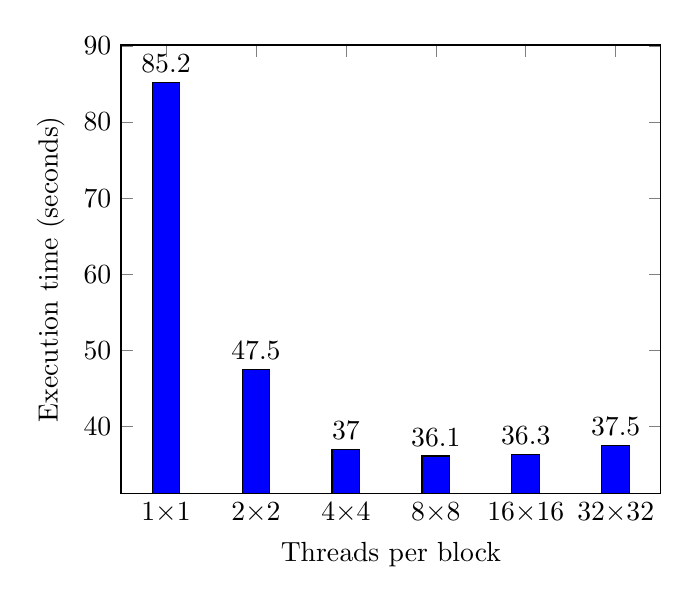
\begin{tikzpicture}

    \begin{axis}[
        ylabel={Execution time (seconds)},
        xlabel={Threads per block},
symbolic x coords={1$\times$1,2$\times$2, 4$\times$4, 8$\times$8, 16$\times$16, 32$\times$32},
        xtick=data,
        nodes near coords={
            \pgfmathprintnumber[precision=1]{\pgfplotspointmeta}
          },
      ]
      \addplot[ybar,fill=blue] coordinates {
(1$\times$1,   85.193986)
(2$\times$2,   47.489448)
(4$\times$4,  37.025578)
(8$\times$8,   36.132327)
(16$\times$16,   36.295435)
(32$\times$32,   37.487930)
        };
    \end{axis}
  \end{tikzpicture}
  \caption{Execution time of different grid configurations for V1}
  \label{fig:executionTimeV1}
\end{figure}

Analyzing this version using the profiling tool \texttt{NVPROF} we can conclude that the majority of execution time is spent in communication between the host and the device, with only  22.19\% of the execution time dedicated to kernel execution. The program spends 41.74\% of time copying data from the host to the device and 36.07\% from the device to the host. The complete results are available at \texttt{results/v1/nvprof\_results}.
From this iteration, we concluded that the better configuration is to use 16$\times$16 threads. We will use this configuration in the next versions.

\subsection{V2 Version --- Better comunication}
In this version, we intend to improve the previous naive implementation, reducing the communication between the host and the device, which we detect to be a big problem in the previous version. In this problem, there aren't any computations needed between the steps so we don't need to transfer the data to the host between steps.

As expected we got a huge improvement in execution time. This version has an average execution time of 2.172697 seconds. Using \texttt{NVPROF} we can see that now the kernel is executing 100.00\% of the total execution time. The full report is in \texttt{results/v2/nvprof\_results}.

We want to understand the impact that this new communication profile is affected by the number of threads so we conduct an analysis similar to the previous one, showing the results in \autoref{fig:executionTimeV2}.

\begin{figure}[ht]
  \centering
  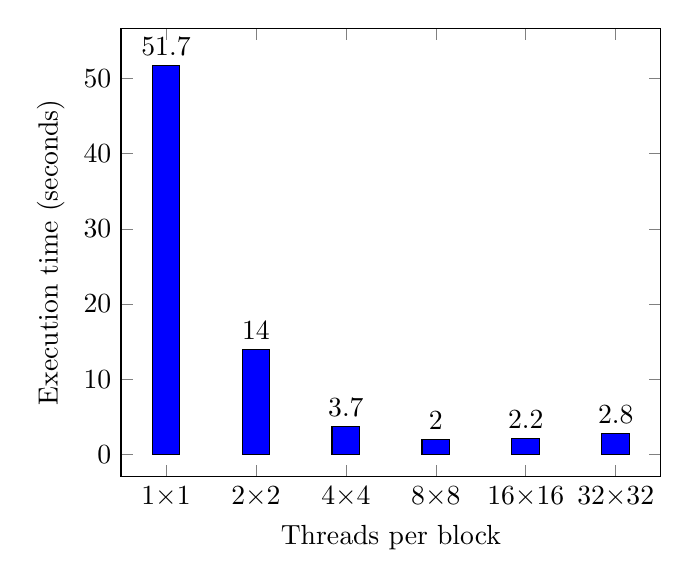
\begin{tikzpicture}

    \begin{axis}[
        ylabel={Execution time (seconds)},
        xlabel={Threads per block},
symbolic x coords={1$\times$1,2$\times$2, 4$\times$4, 8$\times$8, 16$\times$16, 32$\times$32},
        xtick=data,
        nodes near coords={
            \pgfmathprintnumber[precision=1]{\pgfplotspointmeta}
          },
      ]
      \addplot[ybar,fill=blue] coordinates {
(1$\times$1,   51.719873)
(2$\times$2,   13.972750)
(4$\times$4,  3.735481)
(8$\times$8,   2.025430)
(16$\times$16,   2.172697)
(32$\times$32,   2.798723)
        };
    \end{axis}
  \end{tikzpicture}
  \caption{Execution time of different grid configurations for V2}
  \label{fig:executionTimeV2}
\end{figure}
We maintain the use of the 16$\times$16 configuration as the default for this version.

% We decided, from now on, to increase the complexity of the problem by increasing the amount of work, to better spot the improvements. So we define \texttt{numSteps = 1000000}, and maintain the output of the image in the beginning and end.

% With this new parameter, the average execution time is 25.280373 seconds.

\subsection{V3 Version --- Shared Memory}
Looking deeper into our current solution we realize that the same array position is accessed by five different threads, thus revealing a great opportunity for the use of shared memory.

In this version, we take advantage of the shared memory between threads of the same block. Each thread starts by coping a value to the shared memory and after synchronization, the thread computes the designated value.

This version had an average execution time of 2.206946 seconds, which doesn't show any improvement compared with the previous version. This may be because of the overhead introduced by copying each element and the threads' synchronization is not balanced by faster access to the shared memory.


\subsection{V4 Version --- Streams with shared memory}
After analyzing our version with shared memory we decided to add streams to this version despite not expecting any big improvement when working with a small grid.

Our implementation adds streams that allow the device to run as soon as the first partition of our table is downloaded. Since our function works with smaller squares we have a two-dimension cycle in order to copy the necessary data.

We were already expecting the results we got, an average execution time of 2.203838 seconds when using 16 streams (4$\times$4). This time is similar to the time obtained by V3, it's to be expected because of a few factors, which the biggest is that the majority of the time is spent on the execution of steps, so, the time saved in the execution of the first step e relatively small.


\subsection{V5 Version --- Streams}
After V4 we already knew that since we weren't solving any of the major issues listed earlier we would get similar results, however, for the sake of verifying our expectations, we decided that the work implementing the same stream system as before but without the shared memory could be justified.

This version was executed in \texttt{node17} and had an average execution time of 3.369381 seconds not showing any improvements when compared to the V2, that when executed in the same node had an average execution time of 3.355694 seconds.

In conclusion, we confirmed our predictions without any improvements whatsoever.


\subsection{V6 Version --- Streams to copy output}
% V6 comment
We expect streams to prove advantageous when we want the output in intermediate steps, allowing the communication to overlap with the computation of the next step. To perform this analysis we compare the V2 and V6 versions, varying the parameter \texttt{outputEvery} to values of 1000, 100, 10, and 1.

For larger values of \texttt{outputEvery}, we cannot see significant differences revealing that the costs required for synchronization are not balanced by the overlap of communication with synchronization. But with lower values, we have begun to see the advantages of the use of streams. We can see the results in \autoref{fig:v2andv6OutputSteps}.

With the results on every step is where we see the better improvement allowed by streams, in the end of every step we can overlap the execution of the next step with the transfer of the previous result and its writing on a host file.


\begin{figure}[ht]
  \centering
  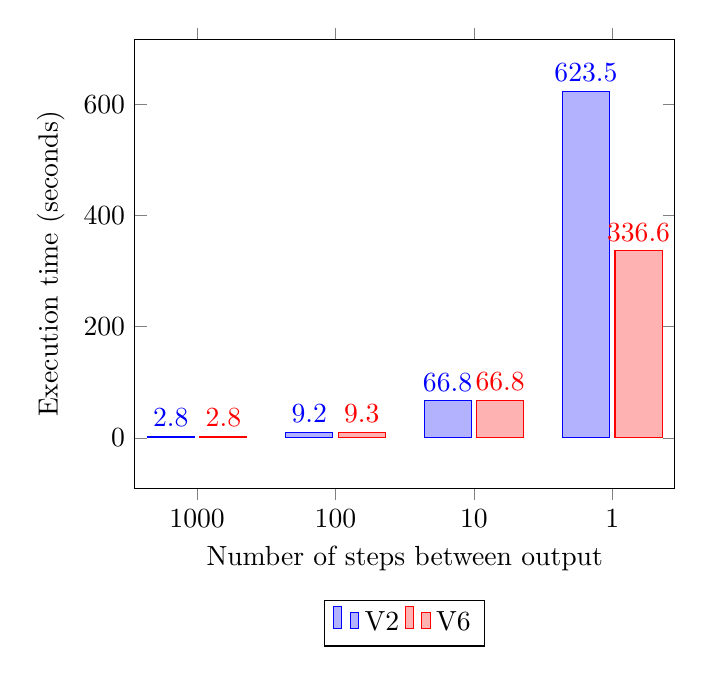
\begin{tikzpicture}
    \begin{axis}[
        ybar,
        enlargelimits=0.15,
        legend style={at={(0.5,-0.25)},
            anchor=north,legend columns=-1},
        ylabel={Execution time (seconds)},
        xlabel={Number of steps between output},
        symbolic x coords={1000, 100, 10, 1},
        xtick=data,
        bar width = 17pt,
        nodes near coords={
            \pgfmathprintnumber[precision=1]{\pgfplotspointmeta}
          },
        % nodes near coords style={font=\tiny},
      ]

      % V2
      \addplot
      coordinates {(1000, 2.792264) (100, 9.190634) (10, 66.757882) (1, 623.521411)};
      % V6 
      \addplot
      coordinates {(1000, 2.758605) (100, 9.334019) (10, 66.824627) (1, 336.616278)};

      \legend{V2,V6}
    \end{axis}
  \end{tikzpicture}
  \caption{Comparing execution time of V2 and V6, varying \texttt{outputEvery}}
  \label{fig:v2andv6OutputSteps}
\end{figure}



Another situation in that streams may be helpful is when we have a larger amount of data to transfer between the host and the device. To prove this hypothesis we vary the grid size and compare the different versions, showing the results in \autoref{fig:v2andv6Grid}.

As we can see the use of streams does not appear to improve the performance when using larger data sets. This may be because the communication time is greater than the execution time of each kernel.


\begin{figure}[ht]
  \centering
  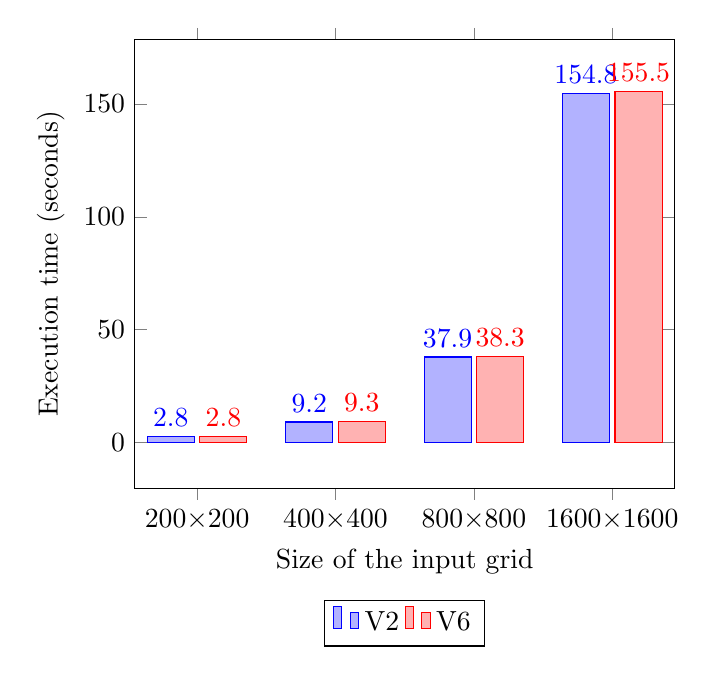
\begin{tikzpicture}
    \begin{axis}[
        ybar,
        enlargelimits=0.15,
        legend style={at={(0.5,-0.25)},
            anchor=north,legend columns=-1},
        ylabel={Execution time (seconds)},
        xlabel={Size of the input grid},
symbolic x coords={200$\times$200, 400$\times$400, 800$\times$800, 1600$\times$1600},
        xtick=data,
        bar width = 17pt,
        nodes near coords={
            \pgfmathprintnumber[precision=1]{\pgfplotspointmeta}
          },
        % nodes near coords style={font=\tiny},
      ]

      % V2
      \addplot
coordinates {(200$\times$200, 2.792264) (400$\times$400, 9.154722) (800$\times$800, 37.918869) (1600$\times$1600, 154.764305)};
      % V6 
      \addplot
coordinates {(200$\times$200, 2.792264) (400$\times$400, 9.309657) (800$\times$800, 38.313756) (1600$\times$1600, 155.506449)};

      \legend{V2,V6}
    \end{axis}
  \end{tikzpicture}
  \caption{Comparing execution time of V2 and V6, varying the input size}
  \label{fig:v2andv6Grid}
\end{figure}

\subsection{V7 and V8 - Streams}

In V7 and V8 we took the first version and developed these versions under the assumption that it would be necessary to copy data from the device to the host and from the host to the device at each step.

To achieve improvements relative to V1 we propose the use of streams. The idea of the two versions is to test the different ways of launching the kernel and the streams, as shown in CUDA documentation\cite{HowOverlapData2012}, and understand how that impacts the performance.

However, we have not been successful in developing these versions, and some errors cause longer execution times and erroneous results. Due to this fact, these versions will be excluded from our analyses.


\subsection{V9 and V10 Versions - More Work per Thread}
Being a bit more creative in our approach for version V9, we decided to have a different evaluation process. In this version, we went back to our V2 and changed it for each thread to process more than a single point of the table. V10 was supposed to do the same as V9 but with the help of shared memory.

The idea was to see if increasing the amount of work and consequently, memory access, makes the use of shared memory justified by improving performance.

Unfortunately, we ran into illegal memory access and we didn't have time to correct our implementations, so we don't have results for these versions.

% Our first attempt was to adapt each thread to process one line of values. This experiment turned out to be a horrible solution with 350+ seconds of execution in the same conditions as the cases above, but as we said this was only the first attempt. The result was surprising because we weren't expecting such a high value but we were it's understandable since we are overworking our threads, with 256 threads per block and 200 lines to process we were making a step work in less than one block, far from maximizing the use of our GPU.

% Finally, our last implementation was to make use of shared memory together with the V9 implementation to make use of the great search speeds when searching a bigger number of values, since starting this memory was also quite a heavy task. This way we were expecting quite an improvement when compared to V9.

\section{Discussion}

Throughout this report, we analyzed many different implementations of the heat equation taking advantage of the GPU.

In \autoref{fig:executionTimeCompare} we can see the execution times of our versions using the same parameters.
Due to a change in the method of measuring execution time and a problem in \texttt{node14} of the DI cluster, it was not possible to run all the versions in the same node. Version V5 was only executed in \texttt{node17}. To better compare the versions we rerun V2 in this node and we show the results of the different versions executed in \texttt{node17} in \autoref{fig:executionTimeCompareNode17}

% TODO atualizar valores
\begin{figure}[ht]
  \centering
\begin{subfigure}[b]{\columnwidth}

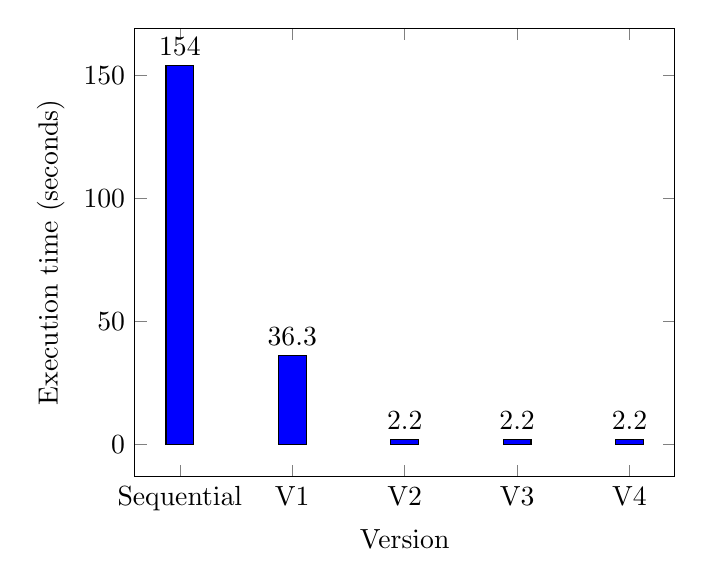
\begin{tikzpicture}
\begin{axis}[
    ylabel={Execution time (seconds)},
    xlabel={Version},
    symbolic x coords={Sequential, V1, V2, V3, V4},
    xtick=data,
    nodes near coords={
        \pgfmathprintnumber[precision=1]{\pgfplotspointmeta}
      },
  ]
  \addplot[ybar,fill=blue] coordinates {
      (Sequential,   153.979491)
      (V1,  36.295435)
      (V2,   2.172697)
      (V3,   2.206946)
      (V4,   2.203838)
    };
\end{axis}
\end{tikzpicture}

\caption{Execution times of sequential version, V1, V1, V3 and V4 in \texttt{node14}}
\label{fig:executionTimeCompareNode14}
  \end{subfigure}
\begin{subfigure}[b]{\columnwidth}
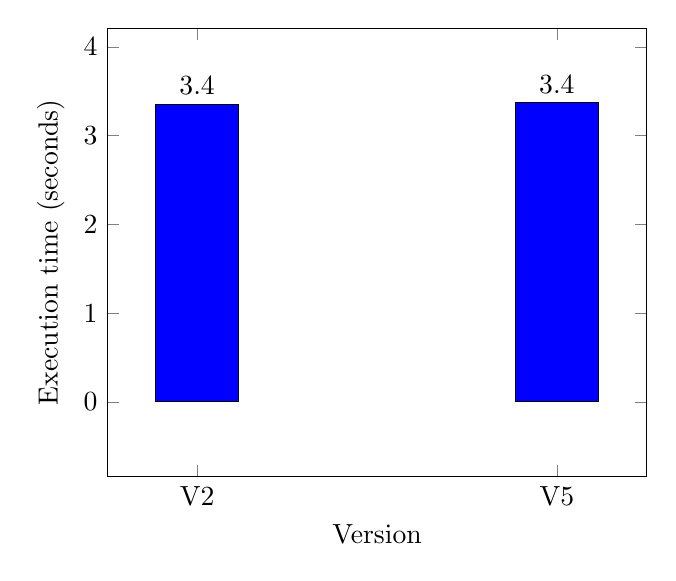
\begin{tikzpicture}

\begin{axis}[
ylabel={Execution time (seconds)},
xlabel={Version},
symbolic x coords={V2, V5},
xtick=data,
ymin = 0,
enlargelimits=0.25,
bar width= 30,
nodes near coords={
\pgfmathprintnumber[precision=1]{\pgfplotspointmeta}
},
]
\addplot[ybar,fill=blue] coordinates {
(V2,   3.355694)
(V5,   3.369381)
};
\end{axis}
\end{tikzpicture}
\caption{Execution times of V2 and V5  \texttt{node17}}
\label{fig:executionTimeCompareNode17}
\end{subfigure}
  \caption{Execution time of the different versions}
  \label{fig:executionTimeCompare}
\end{figure}

With this report, we could see how many strategies influence the performance of a problem and understand that not all solutions are fit for all problems. High-performance computing requires careful analyses of the problem size, structure, and requirements to find the best strategy to parallelize it.

In this problem, and with our implementation we didn't find any advantage in the usage of streams or shared memory, this may due to the fact that the extra work necessary to launch these versions is not compensated by the performance gains. So to this problem, we considered V2 as the best version.

\section{Compilation and Execution Instructions}
Our best version, V2, can be compiled and executed with the following command, from inside the folder \texttt{/proj1}:
\begin{verbatim}
nvcc -o v2 v2.cu && ./v2
\end{verbatim}
This will execute ten iterations to measure the average execution times and the results of the heat equation will be saved in the folder \texttt{images/v2}.


\printbibliography


\end{document}